\subsection{\label{sec:calib.tag}Tagger Timing Calibration}
The timing calibration of the tagger system was performed using the standard procedures. Overall, the quality of the calibration is excellent, showing an overall timing resolution of about $130~ps$, when the tagger time is compared with the RF time. The counter-by-counter alignment can be seen on Fig.~\ref{tagtpho}. The calibration was checked on a run by run basis (Fig.~\ref{tagRun}), and new constants were commissioned when major changes were noticed.  

\begin{figure}[h]
\begin{center}
 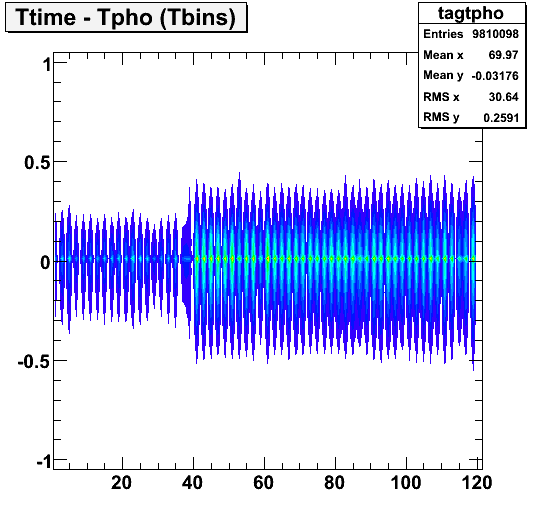
\includegraphics[width=0.45\textwidth]{figures/calib/tag/tagtpho.png}
  \caption{And example of the tagger timing calibration and the T-counter alignment, comparing  the difference between photon time determined from the tagger elements (T-counters, in this particular plot), and photon timing according to the RF. }
  \label{tagtpho}
  \end{center}
\end{figure}


\begin{figure}[h]
\begin{center}
 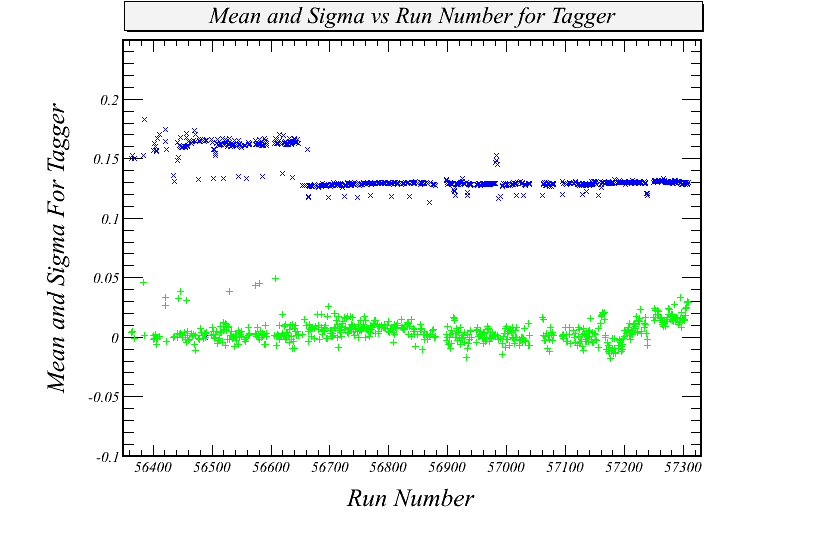
\includegraphics[width=0.45\textwidth]{figures/calib/tag/tagRun.png}
  \caption{The run-by-run behavior of the tagger timing calibration. Overall, the tagger timing resolution is about $130~ps$ for the production runs, and behaves stably throughout the running period.}
  \label{tagRun}
  \end{center}
\end{figure}
